\chapter{Clientes de XRemoteBot}\label{cha:clientes}

La implementación de XRemoteBot para esta tesina incluye tres clientes en distintos
lenguajes de programación: Python, Ruby y Javascript. Este último diseñado para ejecutarse
en el entorno de un navegador web.

Estos clientes tienen distintas características y principalmente el que más
difiere de los demás es el cliente Javascript ya que es una implementación a
ser ejecutada en un navegador web con las restricciones que esto trae, pero
con la ventaja de que
se encuentra integrado con la vista web de XRemoteBot por lo que cuenta con una
vista de la cámara que integra en una misma pantalla la acción de programar del
usuario con el resultado de la ejecución de dicho código.

En general, se intentó mantener el estilo de programación del módulo DuinoBot
original de la forma más fiel posible. En el caso de Javascript por
limitaciones del entorno
no se logró imitar este estilo tan fielmente como en los otros clientes.

\section{Cliente Python}\label{sec:python}
El uso del cliente Python es muy similar al uso directo de los robots con la
biblioteca DuinoBot, aunque la implementación es bastante diferente por el protocolo
subyacente.

El cliente Python utiliza un solo módulo que no pertenece a la biblioteca estándar
de Python: el módulo para acceso a WebSockets
\textit{websocket-client}\footnote{\url{https://pypi.python.org/pypi/websocket-client}}
que cuenta, con una interfaz asincrónica y con una interfaz de ``bajo nivel''
sincrónica similar a la interfaz tradicional de
Sockets\footnote{\url{http://pubs.opengroup.org/onlinepubs/7908799/xns/syssocket.h.html}},
lo que hace más
natural imitar una biblioteca como DuinoBot.

\begin{lstlisting}[language=Python,
caption={Ejemplo con XRemoteBot para Python},label=lst:ejemplo_xremotebot_python]
from xremotebot import *
server = Server('ws://xremotebot.example:8000/api', 'api_key')
robot = Robot(server, server.fetch_robot())
robot.forward(100, 1)
robot.backward(50, 2)
print(robot.getObstacle())
\end{lstlisting}

En el código~\ref{lst:ejemplo_xremotebot_python} se muestra
un script sencillo creado usando el cliente para Python de XRemoteBot. Este
script reserva un robot en la línea 3, luego lo hace avanzar
a velocidad máxima por 1 segundo, lo hace girar a velocidad media
durante 2 segundos y finalmente imprime en pantalla un valor booleano
que indica si existe algún obstáculo enfrente del robot.

Los movimientos, que pueden recibir por parámetro un tiempo de demora,
se implementan en el cliente
utilizando dos mensajes (uno que comienza el movimiento y otro que lo detiene)
y la función \texttt{time.sleep()} de Python,
esta función suspende la ejecución del hilo actual durante el número
de segundos que se envíe como parámetro. De esta
forma
invocar el método \texttt{robot.forward(100, 1)} en el cliente provoca que
el mismo envíe al servidor los mensajes del
código~\ref{lst:ejemplo_xremotebot_python_json} con una pausa de un segundo
entre ellos. Como todos los métodos de movimiento
proveen esta funcionalidad de demora, la misma está implementada en el
\textit{decorator}\footnote{Esto es un decorator de Python, no confundir
con el patrón de diseño. \url{https://www.python.org/dev/peps/pep-0318/}}
\texttt{xremotebot.timed} a fin de evitar la repetición de código.

\begin{lstlisting}[language=Python,
caption={Mensajes generados al invocar \texttt{robot.forward(100, 1)} en
XRemoteBot para Python}, label=lst:ejemplo_xremotebot_python_json]
{
    "entity": "robot",
    "method": "forward",
    "args": [100]
}
# Después de 1 segundo...
{
    "entity": "robot",
    "method": "stop",
    "args": []
}
\end{lstlisting}


\section{Cliente Ruby}\label{ch4:ruby}

Las gemas (en Ruby el formato de habitual de los paquetes de software
se denomina ``gema'' o, en inglés, ``gem''~\citep{thomas_2013})
que proveen soporte para WebSockets en Ruby cuentan con una API
asincrónica que no es adecuada para este proyecto.
Por esto originalmente se analizó incorporar el código del proyecto
\textit{web-socket-ruby}\footnote{\url{https://github.com/gimite/web-socket-ruby}}
al cliente Ruby de XRemoteBot. Este proyecto no ese encuentra empaquetado en
forma de gema, pero provee una API sincrónica que permiría implementar el
cliente Ruby de XRemoteBot
con una interfaz similar a la biblioteca DuinoBot original.
Sin embargo este proyecto no funciona
con servidores modernos de WebSockets. Por ello, en su lugar,
se utilizó la gema \textit{websocket}\footnote{\url{https://github.com/imanel/websocket-ruby}}
que no es una implementación completa
del protocolo, sino que es una biblioteca de bajo nivel que
solamente permite codificar y decodificar mensajes del protocolo, pero no provee
acceso a la red.

Para proveer cierto nivel de abstracción en el acceso a los WebSockets
se implementó la clase
\texttt{WS} que provee la funcionalidad requerida
usando la clase TCPSocket\footnote{\url{http://ruby-doc.org/stdlib-2.1.0/libdoc/socket/rdoc/TCPSocket.html}}
de Ruby para el acceso a la red y
la gema \textit{websocket} para codificar y decodificar los mensajes intercambiados.
Esta implementación se diseñó para que provea una interfaz similar a la de
\textit{websocket-client}\footnote{\url{https://pypi.python.org/pypi/websocket-client}}.

La implementación realizada cuenta con la limitación que por
el momento solamente soporta conexiones inseguras, a futuro es
posible agregar soporte de conexiones seguras usando el módulo
\textit{openssl}\footnote{\url{http://ruby-doc.org/stdlib-2.2.1/libdoc/openssl/rdoc/OpenSSL.html}}.

\begin{lstlisting}[language=Ruby,
caption={Ejemplo usando XRemoteBot para Ruby},
label=lst:ejemplo_xremotebot_ruby]
require 'xremotebot'
server = XRemoteBot::Server.new('xremotebot.example',
                                8000,
                                'api',
                                'api_key')
robot = Robot.new server, server.fetch_robot
robot.forward 100, 1
robot.backward 50, 2
print robot.getObstacle
\end{lstlisting}

El código~\ref{lst:ejemplo_xremotebot_ruby} implementa exactamente la misma funcionalidad que
el el ejemplo en Python visto anteriormente (código~\ref{lst:ejemplo_xremotebot_python}) pero
usando la biblioteca XRemoteBot para Ruby.

\section{Cliente Javascript}\label{sec:javascript}
Como se mencionó con anterioridad, gran parte de las decisiones de diseño de XRemoteBot
se hicieron para permitir la implementación de un cliente Javascript. Sin embargo, aún
tomando estas precauciones, el cliente Javascript resulta ser la más compleja de las
tres implementaciones de clientes desarrolladas.

\subsection{API Javascript y asincronismo}
Dado el hecho
de que Javascript, dentro del entorno de un navegador web se comporta de forma asincrónica,
no fue posible implementar un cliente Javascript cuyo uso se asemeje al de la biblioteca
de Python DuinoBot.

Para ilustrar esta problemática se puede tomar en consideración el
código~\ref{lst:ejemplo_duinobot}
hecho usando DuinoBot en Python y analizar los inconvenientes para replicar
algo similar en Javascript.

\begin{lstlisting}[language=Python,
caption={Ejemplo típico usando DuinoBot},label=lst:ejemplo_duinobot]
from duinobot import *
board = Board()
robot = Robot(board, 10)

robot.forward(100, 1)       # avanza, bloquea la ejecución del script
                            # 1 segundo y luego detiene el robot.

robot.backward(50, 2)       # retrocede, bloquea la ejecución del
                            # script durante 2 segundos y luego
                            # detiene el robot.

print(robot.getObstacle())  # imprime True si hay un obstáculo.
\end{lstlisting}


Las líneas 5 y 8 del código~\ref{lst:ejemplo_duinobot}
no se pueden traducir de forma directa
a Javascript ya que demoran la ejecución del programa
1 y 2 segundos respectivamente, esto es imposible de implementar en
Javascript en el entorno de un navegador sin utilizar la técnica de ``busy
waiting'' o modificar el código para usar la función de Javascript
\texttt{setTimeout()}. La línea 12 tampoco puede transladarse a Javascript
sin grandes modificaciones, ya que requiere enviar un mensaje al servidor
para pedirle los datos del sensor, esperar la respuesta y retornarla, todo
esto no es posible con WebSockets en el navegador ya que su API es asincrónica.

Utilizar la técnica ``busy waiting'' en el navegador no sería adecuado ya que
normalmente los navegadores utilizan un solo thread por pestaña y esto
bloquearía al navegador al menos en la pestaña actual. Por otro lado
el uso de \texttt{setTimeout()} puede servir para implementar las líneas
5 y 8 pero no la línea 12 ya que no es posible determinar el tiempo
de respuesta del servidor.

Como se menciona en el la sección~\ref{sec:websockets}, el servidor
utiliza WebSockets como protocolo de transporte.
La API de WebSockets disponible en los navegadores web es asincrónica y
está basada en el uso de ``callbacks''
que se ejecutan ante distintos eventos~\citep{wang_2013}.
Para utilizar un WebSocket usando esta API es necesario
redefinir una serie de atributos de la instancia del WebSocket,
asignándoles las funciones que se
desea ejecutar ante cada cambio de estado en el
WebSocket~\citep{websocket_2014}:
\begin{description}
    \item[\texttt{WebSocket\#onopen()}:] se ejecutará cuando
    la conexión esté establecida.
    \item[\texttt{WebSocket\#onerror()}:] se ejecutará ante un error en
    la conexión.
    \item[\texttt{WebSocket\#onclose()}:] se ejecutará si la conexión
    se cierra.
    \item[\texttt{WebSocket\#onmessage()}:] se ejecutará al recibir un
    mensaje desde el servidor, recibe como argumento el mensaje
    enviado por el servidor.
\end{description}

Para proveer una interfaz lo más parecida posible a la de DuinoBot,
para implementar
las demoras al invocar a mensajes como \texttt{Robot\#forward()} y
\texttt{Robot\#backward()}, y para implementar mensajes que dependen
del valor de respuesta del servidor como \texttt{Robot\#getObstacle()}
se utilizó el objeto de Javascript \texttt{Promise} en conjunto con
algunas modificaciones en el servidor y en el protocolo que proveen
una solución de alto nivel en comparación con el uso directo de
la API de WebSockets. Esto se describe en la sección~\ref{sec:promises}.

\subsection{Promises}\label{sec:promises}

Para proveer una API lo más parecida posible a DuinoBot sin
tener la capacidad de demorar la ejecución del código hasta que
llegue la respuesta de las peticiones, se investigó la API
\textit{Promise}~\citep{ECMA-262} de ECMAScript 6 que permite modelar
esta espera de una forma razonablemente intuitiva.

Si bien el objeto \textit{Promise} está en proceso de estandarización,
los navegadores Google Chrome, Firefox, Internet Explorer, Opera y Safari lo
soportan\footnote{\url{https://developer.mozilla.org/en-US/docs/Web/JavaScript/Reference/Global_Objects/Promise}}.

Los objetos \textit{Promise} se utilizan para obtener valores resultantes
de cómputos asincrónicos, como es el caso de la respuesta a una petición
hecha con WebSockets. La interfaz de \textit{Promise} no permite programar
los robots en Javascript con una interfaz idéntica a la usada al programar
los robots con la biblioteca DuinoBot, pero es relativamente fácil de
utilizar y ante la imposibilidad de demorar la ejecución del código
Javascript provee una alternativa
relativamente simple en comparación con el uso directo de la interfaz
de los objetos \texttt{WebSocket}.

Los objetos \textit{Promise} se instancian pasándoles como argumento una
función que a su vez recibe 2 argumentos: \texttt{resolve} y \texttt{reject}.
El primer argumento ``cumple'' o ``resuelve'' la promesa y el segundo la
``rechaza''.
Las ``promesas'' tienen dos métodos: \texttt{then} y \texttt{catch} que se
ejecutan cuando la promesa se ``cumple'' o se ``rechaza'' respectivamente.

\subsubsection{Una primer implementación}
Usando esta API se implementó una primer versión de XRemoteBot para Javascript
donde cada mensaje enviado al servidor retorna una instancia de \textit{Promise}.
El código~\ref{lst:ejemplo_xremotebot_javascript} muestra una implementación
en Javascript del ejemplo visto en el código~\ref{lst:ejemplo_duinobot}.

\begin{lstlisting}[language=C,
caption={Ejemplo de XRemoteBot en Javascript},
label=lst:ejemplo_xremotebot_javascript]
var server = new Server('xremotebot.example:8000', 'api-key');
server.onConnect(function(){
    server.fetch_robot().then(function(robot_obj){
        var robot = new Robot(server, robot_obj);
        robot.forward(100, 1).then(function(){
            robot.backward(50, 2).then(function(){
                robot.getObstacle().then(function(obstacle){
                    println(obstacle);
                })
            })
        })
    });
});
\end{lstlisting}

Como se puede ver, después de cada acción bloqueante, es decir cada método que
provoque una demora y de cada método que retorne un valor útil, como
\texttt{Robot\#getObstacle()}, se invoca el método \texttt{Promise\#then()} con
una función anónima como argumento. Esta función, que se pasa por argumento al
método \texttt{Promise\#then()}, se ejecutará si la \textit{Promise} se
``resuelve''. En el caso de
XRemoteBot la \textit{Promise} se ``resuelve'' cuando el servidor
responde al mensaje que generó la \textit{Promise}.

\begin{lstlisting}[language=C,
caption={Ejemplo simplificado de la implementación de XRemoteBot con
Promises dentro del constructor Server en xremotebot.js},
label=lst:ejemplo_xremotebot_javascript_promises]
this.send_ws_msg = function(msg){
    var promise;
    this.msg_id++;
    promise = new Promise(function(resolve, reject){
        that.pending_msgs[msg_id] = {resolve: resolve, reject: reject};
    });
    msg['msg_id'] = msg_id;
    that.ws.send(JSON.stringify(msg));
    return promise;
}
// ...
this.ws.onmessage = function(msg){
    msg = JSON.parse(msg.data);
    if (msg['msg_id'] !== undefined){
        var executor = that.pending_msgs[msg['msg_id']];
        delete that.pending_msgs[msg['msg_id']];
        if (msg.response === 'value'){
            executor.resolve(msg.value);
        }
        else{
            executor.reject(msg.message);
        }
    }
};
\end{lstlisting}

Esta implementación se logró incluyendo en los mensajes un campo
\texttt{msg\_id} que identifica, para cada instancia de WebSocket, a
cada mensaje de forma unívoca. A su vez el servidor, al encontrar este
campo en un mensaje, lo copia sin modificarlo a la respuesta correspondiente
al mismo. Del lado del cliente, por cada instancia de WebSocket se mantiene
una colección de las promesas correspondientes
a cada \texttt{msg\_id} y se las gestiona desde la función
\texttt{WebSocket\#onmessage()} ``resolviéndolas'' o ``rechazándolas'' según
se reciba como respuesta un valor o un error. El
código~\ref{lst:ejemplo_xremotebot_javascript_promises} muestra una versión
simplificada de esta primer implementación.

Cada método de XRemoteBot para Javascript que involucre enviar un mensaje
retornará entonces una ``promesa'', por lo que habrá que tener en cuenta
invocar a ``then()'' o a ``catch()'' cuando es necesario
utilizar el valor retornado por el servidor o determinar si la ejecución fue exitosa.

\subsubsection{Una versión mejorada}

Evidentemente la forma de programar del ejemplo visto en el
código~\ref{lst:ejemplo_xremotebot_javascript}
resulta engorrosa y poco práctica.
Por esto se modificó el cliente Javascript para que no envíe un nuevo mensaje hasta
que el mensaje anterior haya recibido una respuesta. Esto se implementó usando
identificadores secuenciales para los mensajes de forma que se pueda verificar si
el mensaje previo tuvo respuesta y una cola para demorar a los mensajes que aún no
pueden enviarse.

\begin{lstlisting}[language=C,
caption={Ejemplo de XRemoteBot en Javascript con empleo de una cola para
serializar mensajes},
label=lst:ejemplo_xremotebot_javascript_cola]
var server = new Server('xremotebot.example:8000', 'api-key');
server.onConnect(function(){
    server.fetch_robot().then(function(robot_obj){
        var robot = new Robot(server, robot_obj);
        robot.forward(100, 1);
        robot.backward(50, 2);
        robot.getObstacle().then(function(obstacle){
            println(obstacle);
        });
    });
});
\end{lstlisting}

El atributo \texttt{Server\#delayed} en \texttt{xremotebot.js} mantiene la cola
de mensajes demorados.
Cuando el servidor contesta un mensaje previo se toma otro mensaje
de la cola (si lo hubiere) y se lo envía al servidor. De esta manera,
se garantiza la demora necesaria entre la ejecución de cada método
del robot. Sin embargo, para obtener los valores de retorno de los métodos,
como en el caso de los métodos de acceso a los sensores, sigue siendo
necesario el uso del método \texttt{Promise\#then}. A pesar de esto último,
como se puede ver en el código~\ref{lst:ejemplo_xremotebot_javascript_cola},
con estas modificaciones es posible hacer que el cliente Javascript
tenga una API más limpia y usable, esta última versión es la definitiva
para este trabajo.

\subsubsection{Alternativas al uso de promises}

Una solución alternativa para lograr imitar tanto como sea posible la
API de DuinoBot puede ser utilizar un intérprete Javascript implementado en
Javascript como
JS-Interpreter\footnote{\url{https://github.com/NeilFraser/JS-Interpreter}},
pero requeriría modificar el intérprete para lograr una ejecución paso a paso
controlada por el flujo de mensajes a través de la conexión con WebSockets.
Además de agregar complejidad, este tipo de intérpretes no accede a un entorno
completo como lo hace el intérprete incorporado en los navegadores y puede
tener incompatibilidades o funcionalidades no implementadas, en este caso
por ejemplo JS-Interpreter no soporta interrupciones y no puede interactuar
directamente con DOM. Otra opción es
Hypnotic\footnote{\url{http://coolwanglu.github.io/hypnotic/web/demo.html}}
que utiliza el intérprete Narcissus y provee una función \texttt{sleep()} que
demora la ejecución del código como se desea para este proyecto, pero el
inconveniente de Hypnotic es que por el momento solamente funciona en el
navegador
Firefox\footnote{\url{https://github.com/coolwanglu/hypnotic/wiki\#limitations}}.


\subsection{Interacción con el navegador, DOM y JQuery}

Dado que el cliente Javascript se ejecuta en el entorno de un navegador web es posible
interactuar con el árbol DOM de la página. Por ejemplo modificando sus nodos.
Y dado que la interfaz web utiliza
JQuery\footnote{\url{http://jquery.com}}
esta biblioteca también está disponible
para los usuarios, pudiendo hacer por ejemplo un script que pide los valores
de los sensores de línea cada 500 milisegundos y los muestra en el título de la
página usando JQuery para manipular el árbol DOM como se ve en el
código~\ref{lst:ejemplo_dom_title}, el resultado se puede ver en la
figura~\ref{fig:ejemplo_web_sensor}.

\begin{lstlisting}[language=C,
caption={Manipulación de DOM con JQuery desde
XRemoteBot para Javascript},
label={lst:ejemplo_dom_title}]
var server = new Server('ws://localhost:8000/api',
                        '97385401-3874-439c-b01b-df94349d888a');
server.onConnect(function(){
    server.fetch_robot().then(function(robot_obj){
        var robot = new Robot(server, robot_obj);
        setInterval(function(){
            robot.getLine().then(function(line){
                $('title').text('Sensor de línea: ' + line);
            });
        }, 500);
    });
});
\end{lstlisting}

\begin{figure}
    \centering
    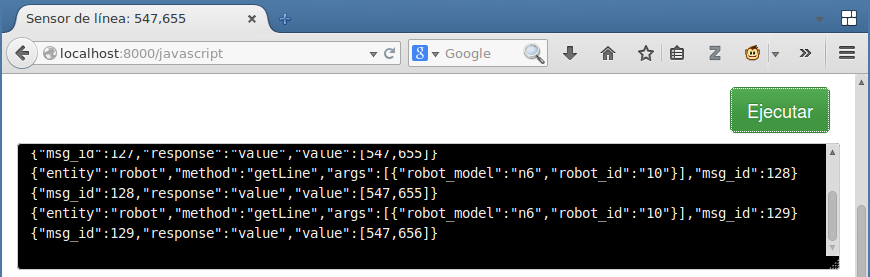
\includegraphics[width=1\textwidth]{figures/ejemplo_web_sensor}
    \caption{Resultado de la ejecución del código~\ref{lst:ejemplo_dom_title}}
    \label{fig:ejemplo_web_sensor}
\end{figure}

\begin{lstlisting}[language=C,
caption={Implementación de \texttt{getObstacle()} con ``promesas''},
label=lst:promises_get_obstacle]
robot.getObstacle().then(function(hay_obstaculo){
    if (hay_obstaculo.value){
        console.log("Hay un obstáculo al frente");
    }
    else {
        console.log("No hay obstáculos");
    }
});
\end{lstlisting}

El código~\ref{lst:promises_get_obstacle} utiliza \texttt{console.log},
para mostrar el valor del sensor de obstáculos en la consola de depuración
del navegador.



\lstinputlisting[language=C,
    caption={Manejo de errores en XRemoteBot para Javascript},
label=lst:promises_catch]{ejemplos/ejemplo_catch.js}


El código~\ref{lst:promises_catch} muestra un ejemplo del manejo de errores
utilizando la función \texttt{catch()}. El ejemplo reserva un robot y
le pide periódicamente el valor de su sensor de obstáculos, si la petición tiene
éxito pone el valor como título de la página, en cambio si la petición falla
(por ejemplo porque expira la reserva) se muestra un mensaje de error.
Este ejemplo combina el acceso
a las funciones del navegador como \texttt{alert()} y \texttt{setInterval()},
el uso de JQuery y la manipulación del árbol DOM.

\noindent \begin{minipage}{0.75\textwidth}
    \hskip 1.5em En un ejemplo más avanzado de uso de DOM y JQuery podría plantearse como
    actividad agregar una botonera para controlar a los robots haciendo clic.
    El código~\ref{lst:botones} muestra una posible solución a esa actividad,
    agregando los botones debajo del área de streaming de video y la
    figura~\ref{fig:botones} muestra el resultado de ejecutar este código.
\end{minipage}
\begin{minipage}{0.25\textwidth}
        \centering
        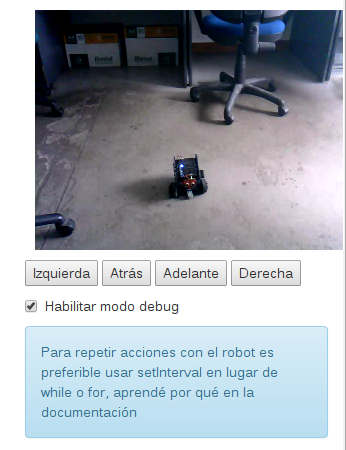
\includegraphics[width=\textwidth]{figures/botones}
        \captionof{figure}{Botonera creada en el código~\ref{lst:botones}}
        \label{fig:botones}
        \vspace{1em}
\end{minipage}

\lstinputlisting[language=C,
    caption={Agregar botones debajo del área de video usando JQuery},
label=lst:botones]{ejemplos/botones.js}



\subsection{Interfaz web y streaming de video}

La interfaz web de XRemoteBot
que está pensada principalmente para los casos
de uso donde los clientes están en una ubicación geográfica distinta a la de
los robots, provee login, acceso a la visualización y renovación de una
clave alfanumérica única por cada usuario denominada \textit{API key} que
permite reservar y controlar los robots sin la necesidad de exponer el nombre
de usuario y contraseña, y una página que permite ver los robots en vivo por
video opcionalmente controlándolos con un script Javascript
(figura~\ref{fig:interfaz_web}),

\begin{figure}
    \centering
    \begin{subfigure}[m]{0.55\textwidth}
        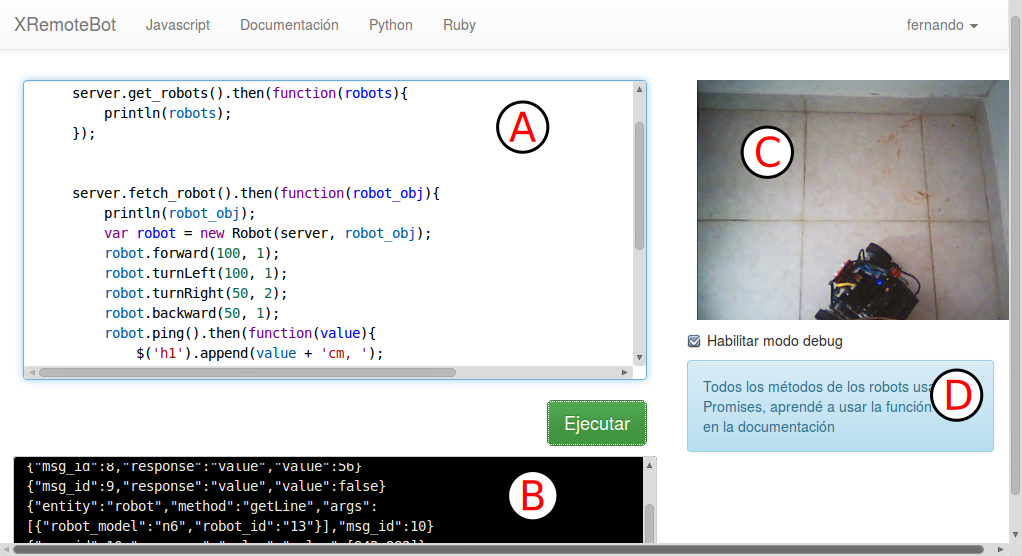
\includegraphics[width=1\textwidth]{figures/xremotebot_gui}
    \end{subfigure}\hskip 0.5em%
    \begin{subfigure}[m]{0.4\textwidth}
        \begin{description}
            \item[A:] área de texto para codificar.
            \item[B:] área que simula una consola. Los programas
                puedan imprimir texto en este área.
            \item[C:] transmisión
                de video. Muestra los robots en tiempo real.
            \item[D:] caja de ``tips'' o consejos.
        \end{description}
    \end{subfigure}
    \caption{Interfaz web de XRemoteBot}
    \label{fig:interfaz_web}
\end{figure}

Esta interfaz provee un sistema para crear usuarios nuevos, obtener las
API key y acceso a la documentación básica para trabajar con XRemoteBot
desde cualquiera de los tres clientes implementados.

La interfaz web fue pensada principalmente para ser utilizada en conjunto
 con el cliente
Javascript, aunque puede ser accedida sin problemas aún si se usa
otro de los clientes para poder visualizar los robots a través del
streaming de video. Provee un área de texto para escribir los scripts a
ejecutar.
Esta área de texto es creada con
CodeMirror\footnote{\url{https://codemirror.net/}}
que provee resaltado de sintaxis y manejo de los eventos de teclado para
que, al presionar \textit{Tab}, el editor indente el código en lugar de saltar a otro
elemento de la página como harían los navegadores por defecto.

Otra área de texto en la parte inferior
simula la salida de una terminal, en la misma
se pueden ver mensajes de log generados con la función
\texttt{rblog} que pueden ser habilitados o deshabilitados con la opción
``habilitar modo debug''
 y mensajes impresos con la función \texttt{println}.
Ambas funciones pueden imprimir, además de cadenas de texto, objetos. Estos últimos
se convierten a cadenas de texto usando la función \texttt{JSON.stringify()}.

Un área de video destinada a emisiones en vivo que muestren la posición
del robot, el mismo no requiere ningún plugin ya que se utilizó
\texttt{jsmpeg}\footnote{\url{https://github.com/phoboslab/jsmpeg}}
que permite emitir video en vivo usando WebSockets y renderizarlo
en el navegador en un elemento Canvas, de esta manera se logró tener
video en vivo utilizando características estándar de HTML5.
